\documentclass[11pt,letterpaper]{article}

\usepackage[margin=1in]{geometry}
\usepackage{amsmath,amssymb,amsthm}
\usepackage{mathtools}
\usepackage{booktabs}
\usepackage{enumitem}
\usepackage{hyperref}
\usepackage[dvipsnames]{xcolor}
\usepackage{titlesec}
\usepackage{microtype}
\usepackage{parskip}
\usepackage{tikz}
\usetikzlibrary{arrows.meta,positioning,calc,fit,backgrounds}

\hypersetup{colorlinks=true, linkcolor=NavyBlue, citecolor=NavyBlue, urlcolor=NavyBlue}
\titleformat{\section}{\large\bfseries}{\thesection}{1em}{}
\titleformat{\subsection}{\normalsize\bfseries}{\thesubsection}{1em}{}
\titleformat{\subsubsection}{\normalsize\itshape}{\thesubsubsection}{1em}{}

\newcommand{\caveat}[1]{\par\smallskip\noindent\textcolor{gray}{\textit{Caveat:} #1}\smallskip}
\newcommand{\pp}{\,\text{pp}}
\newcommand{\bfp}{\mathbf{p}}
\newcommand{\bfz}{\mathbf{z}}
\newcommand{\bfy}{\mathbf{y}}
\newcommand{\bfd}{\mathbf{d}}
\newcommand{\bfb}{\mathbf{b}}
\newcommand{\cS}{\mathcal{S}}
\newcommand{\cM}{\mathcal{M}}
\newcommand{\R}{\mathbb{R}}

\begin{document}

\begin{center}
{\LARGE\bfseries Neural Field Perceiver}\\[6pt]
{\large Cross-Patient Speech Decoding from Intra-Operative $\mu$ECoG\\via Reprojection-Supervised Spatial Alignment}\\[12pt]
{\normalsize Ben Tang \quad\textbar\quad Greg Cogan Lab, Duke University}\\[4pt]
{\normalsize April 2026 \quad\textbar\quad Problem Framing + Architecture Design}
\end{center}

\medskip\noindent\rule{\textwidth}{0.4pt}\medskip

\tableofcontents
\newpage

%% ====================================================================
%%  PART I: PROBLEM FRAMING
%% ====================================================================

\part{Problem Framing}

\section{The Physical Problem}

Each patient's micro-electrocorticography ($\mu$ECoG) array is a \textbf{sparse spatial sample} of neural activity over the cortical surface during speech production. The array is placed subdurally over left ventral sensorimotor cortex (vSMC) during surgery, and its position in standardized brain space (MNI-152) is determined post-hoc via electrode reconstruction.

\subsection{The cortical surface, not free 3D space}

The cortex is a folded two-dimensional sheet. Let $\cS$ denote the cortical surface embedded in $\R^3$. The high-gamma analytic amplitude (HGA, 70--150\,Hz) is a function on this surface:
\begin{equation}
a: \cS \times \R \to \R
\end{equation}
For patient $i$ with $N_i$ electrodes at cortical surface positions $\{\bfp_j^{(i)}\}_{j=1}^{N_i} \subset \cS$, we observe:
\begin{equation}\label{eq:observation}
d_j^{(i)}(t) = a\bigl(\bfp_j^{(i)},\; t\bigr) + \epsilon_j^{(i)}(t)
\end{equation}
In practice, we approximate surface positions with 3D MNI coordinates. Euclidean distance in MNI does not equal geodesic distance on the cortical surface---electrodes on opposite sulcal banks may be close in 3D but functionally distant. For $\mu$ECoG arrays on exposed cortex, the local patch is approximately planar, so within-array Euclidean distances are reasonable.

\textbf{The decoding problem.} Given $\{d_j^{(i)}(t)\}$ at approximately known positions, infer the phoneme sequence $\bfy = (y_1, y_2, y_3)$.

\textbf{The cross-patient problem.} Train on patients $\{1, \ldots, K\}$, decode for held-out patient $K{+}1$ whose electrodes sample the surface at different positions.

\subsection{What makes this hard}

\begin{table}[ht]\centering\small
\begin{tabular}{@{}lll@{}}
\toprule
\textbf{Factor} & \textbf{Quantity} & \textbf{Implication} \\
\midrule
Electrodes per patient & 63--201 & Sparse sampling \\
Electrode spacing & ${\sim}2$\,mm & Finer than registration accuracy \\
Array offset across patients & 15--25\,mm & Different cortical regions sampled \\
Correspondence uncertainty & Several mm & Coordinate alignment is approximate \\
Tumor mass effect (6/12 patients) & Variable & Macroscopic cortical warping \\
Trials per patient & 46--178 & Small-data regime \\
Total utterance per patient & ${\sim}1$\,min & Insufficient for per-patient SSL \\
\bottomrule
\end{tabular}
\end{table}


\section{The Shared Dynamics Hypothesis}

We decompose:
\begin{equation}\label{eq:decomposition}
\boxed{a^{(i)}(\bfp, t) = f\bigl(T_i(\bfp),\; t;\; \bfy\bigr) + r^{(i)}(\bfp, t)}
\end{equation}
\begin{itemize}[leftmargin=2em]
\item $f(\cdot, t; \bfy)$: \textbf{shared neural field}---the spatiotemporal pattern that $\bfy$ produces in canonical cortical space.
\item $T_i: \cS_i \to \cS_{\text{canonical}}$: \textbf{patient-specific spatial transform}. MNI normalization estimates $T_i$, imperfectly.
\item $r^{(i)}$: \textbf{patient-specific residual}---fine-grained neural organization, signal characteristics, pathology.
\end{itemize}

\subsection{Evidence hierarchy}

\subsubsection{Externally established}
Per-patient input + shared backbone is optimal (Singh 2025, $N{=}25$, PER 0.49 vs.\ 0.57; Willett 2023, per-day affine + shared GRU). Articulatory somatotopy exists in vSMC (Metzger 2023, Bouchard 2013). MNI coordinates enable cross-patient ECoG transfer (Chen 2025 SwinTW, 43+9 subjects, PCC 0.765). Motor cortex manifold dynamics preserved across individuals (Safaie 2023) and stable over time (Gallego 2020). Articulatory features robustly encoded in vSMC (Wu 2025).

\subsubsection{Internally observed}
LOPO achieves PER 0.762 on S14 (vs.\ per-patient 0.737). Articulatory bottleneck head improves cross-patient decoding. Multi-scale temporal encoding (stride 3+5+10) is the best architectural improvement ($0.766 \to 0.750$). 55 experiments converge to PER 0.750--0.780. All domain adaptation methods (DANN, CORAL, CCA) provide zero benefit.

\subsubsection{Working hypotheses}
The ${\sim}0.76$ convergence partly reflects spatial alignment limitations (not isolated from data scarcity or S14-specific effects). MNI coordinates will improve decoding (depends on registration accuracy and whether alignment is binding). Cross-task pooling (Duraivel 2025) is a high-value, low-risk path to more data.


\section{The Neural Manifold Connection}\label{sec:manifold}

\subsection{Two views, one bridge}

The cortical field model and the neural manifold hypothesis are dual descriptions. The bridge is the \textbf{latent articulatory state} $\bfz(t) \in \R^k$:
\begin{equation}\label{eq:obs-function}
\boxed{d_j^{(i)}(t) = g\bigl(\bfp_j^{(i)},\; \bfz(t)\bigr) + \epsilon_j^{(i)}(t)}
\end{equation}
where $g: \cS \times \R^k \to \R$ is a \textbf{shared observation function}---the somatotopic map. Electrodes over lip motor cortex respond to lip-state variables; electrodes over tongue cortex to tongue-state variables.

The dynamics on the manifold are phoneme-determined:
\begin{equation}\label{eq:dynamics}
\dot{\bfz}(t) = h\bigl(\bfz(t);\; \bfy\bigr)
\end{equation}

\subsection{The factorization is the key insight}

Combining the shared dynamics hypothesis with the manifold hypothesis: the shared field $f(\bfp, t; \bfy)$ factorizes as $g(\bfp, \bfz(t))$, separating space from time through a low-dimensional bottleneck. Instead of learning an arbitrary spatiotemporal function, the model learns:
\begin{enumerate}[leftmargin=2em]
\item A spatial function $g$: how each brain position encodes articulatory features (the somatotopic map).
\item A dynamical system $h$: how the articulatory state evolves during speech.
\end{enumerate}

\subsection{Articulatory manifold dimensionality}

The manifold has physical meaning. For our 9 phonemes:

\begin{table}[ht]\centering\small
\begin{tabular}{@{}llc@{}}
\toprule
\textbf{Contrast} & \textbf{Phonemes distinguished} & \textbf{Dim.}\\
\midrule
Place of articulation & labial (b,p,v) vs.\ velar (g,k) & ${\sim}2$ \\
Manner & stop vs.\ fricative vs.\ vowel & ${\sim}2$ \\
Voicing & voiced (b,g,v) vs.\ voiceless (k,p) & ${\sim}1$ \\
Vowel height/backness & (a,\ae,i,u) contrasts & ${\sim}2$ \\
\midrule
\textbf{Total effective dimension} & & ${\sim}\mathbf{5\text{--}8}$ \\
\bottomrule
\end{tabular}
\end{table}

This is far below electrode count (63--201): the decoding problem is well-posed.

\subsection{Cross-patient transfer as manifold alignment}

Each patient's array gives a different projection of the shared manifold:
$\bfd^{(i)}(t) \approx W^{(i)} \bfz(t) + \boldsymbol{\epsilon}^{(i)}$,
where $W^{(i)} \in \R^{N_i \times k}$ is determined by electrode positions. MNI coordinates provide the geometric relationship between these projections a priori, rather than requiring post-hoc alignment.


\section{Decomposing Cross-Patient Variation}

\subsection{The spatial transform}

\begin{equation}
T_i(\bfp) = A_i \cdot \bfp + \bfb_i + \delta_i(\bfp)
\end{equation}
$A_i$: rigid/affine (corrected by MNI normalization). $\bfb_i$: translation (15--25\,mm array offsets). $\delta_i$: nonlinear residual including \textbf{tumor mass effect}---a geometric mapping error that physically displaces the somatotopic map.

\subsection{Inter-subject correspondence uncertainty}

Not a fixed constant. Sources: native-space localization (sub-mm), brain shift correction (variable), atlas warping (dominant). Net result: several mm for healthy anatomy, more near tumors.

\subsection{Resolution mismatch $\Rightarrow$ dual spatial encoding}

\begin{table}[ht]\centering\small
\begin{tabular}{@{}llll@{}}
\toprule
\textbf{Scale} & \textbf{Resolution} & \textbf{Best encoded by} & \textbf{What it captures}\\
\midrule
Cross-patient & ${\sim}10$--$15$\,mm & MNI coordinates & Articulatory somatotopy\\
Intra-patient local & ${\sim}2$\,mm & Grid topology & Fine-grained spatial patterns\\
\bottomrule
\end{tabular}
\end{table}


\section{What Our Experiments Reveal}

\textbf{Evaluation recipe dominates:} training improvements ${\sim}7\pp$, evaluation improvements ${\sim}6.5\pp$ (weighted $k$-NN, TTA, articulatory head, best-of per fold). \textbf{Multi-scale temporal validated:} stride 3+5+10 is best architecture ($-1.6\pp$). \textbf{SSL carries partial structure:} JEPA + LP-FT achieves 0.797 (vs.\ 0.854 basic). \textbf{The ${\sim}0.76$ wall:} 55 experiments converge; cannot attribute to a single bottleneck without population-level evaluation.


%% ====================================================================
%%  PART II: THE MULTI-VIEW RECONSTRUCTION ANALOGY
%% ====================================================================

\part{The Multi-View Reconstruction Analogy}

\section{From 3D Pose Estimation to Neural Field Decoding}\label{sec:analogy}

The cross-patient decoding problem has a precise structural analog in computer vision: \textbf{fitting a parametric 3D model to 2D observations from multiple viewpoints}. This analogy, inspired by holistic performance capture approaches (Hewitt et al., 2024, arXiv:2410.11520), motivates the reprojection loss that is central to our architecture.

\subsection{The pose estimation setup}

In 3D human pose estimation (e.g., fitting SMPL to 2D keypoints):
\begin{enumerate}[leftmargin=2em]
\item A \textbf{parametric 3D model} (SMPL) encodes human body structure, parameterized by pose $\theta$ and shape $\beta$.
\item A \textbf{camera} projects 3D model vertices to 2D image coordinates via known projection function $\pi$.
\item We observe \textbf{2D keypoint detections} $\{x_j\}$---sparse, noisy projections of the 3D model.
\item The \textbf{reprojection loss} $\sum_j \|x_j - \pi(V_j(\theta, \beta))\|^2$ drives optimization of pose and camera parameters.
\end{enumerate}

\subsection{The mapping}

\begin{table}[ht]\centering\small
\begin{tabular}{@{}p{0.42\textwidth}p{0.02\textwidth}p{0.48\textwidth}@{}}
\toprule
\textbf{3D Pose Estimation} & & \textbf{Neural Field Decoding} \\
\midrule
3D body model (SMPL mesh) & $\leftrightarrow$ & Shared neural field $g(\bfp, \bfz)$ on cortex \\[3pt]
Pose parameters $\theta$ (joint angles) & $\leftrightarrow$ & Articulatory state $\bfz(t)$ (vocal tract config.) \\[3pt]
Shape parameters $\beta$ (body proportions) & $\leftrightarrow$ & Patient embedding $e^{(i)}$ (neural residual) \\[3pt]
Camera extrinsics $[R \mid t]$ & $\leftrightarrow$ & MNI offset $\Delta^{(i)}$ (registration correction) \\[3pt]
Camera intrinsics $K$ & $\leftrightarrow$ & Per-patient gain/bias (signal scaling) \\[3pt]
2D keypoint observations $x_j$ & $\leftrightarrow$ & Electrode observations $d_j^{(i)}(t)$ \\[3pt]
Projection function $\pi(\cdot)$ & $\leftrightarrow$ & Observation function $g(\cdot)$ \\[3pt]
Keypoint visibility/occlusion & $\leftrightarrow$ & Dead/masked electrodes \\[3pt]
\textbf{Reprojection loss} $\|\pi(V) - x\|^2$ & $\leftrightarrow$ & \textbf{Reprojection loss} $\|g(\bfp{+}\Delta, \hat{\bfz}) - d\|^2$ \\
\bottomrule
\end{tabular}
\end{table}

\subsection{The multi-view extension}

The analogy deepens when we consider multi-patient training as \textbf{multi-view 3D reconstruction}:

\begin{table}[ht]\centering\small
\begin{tabular}{@{}p{0.45\textwidth}p{0.02\textwidth}p{0.45\textwidth}@{}}
\toprule
\textbf{Multi-View Reconstruction} & & \textbf{Multi-Patient Neural Field} \\
\midrule
Multiple cameras observe the same 3D scene from different viewpoints & $\leftrightarrow$ & Multiple patients ``observe'' the same cortical dynamics from different electrode positions \\[6pt]
Each camera has own extrinsics $[R_i \mid t_i]$ & $\leftrightarrow$ & Each patient has own offset $\Delta^{(i)}$, embedding $e^{(i)}$ \\[6pt]
3D structure is \textbf{shared}; only viewpoints differ & $\leftrightarrow$ & Neural field $g$ is \textbf{shared}; only electrode positions differ \\[6pt]
Joint optimization: 3D structure + all camera params & $\leftrightarrow$ & Joint optimization: neural field + all patient params \\[6pt]
More cameras $=$ better reconstruction & $\leftrightarrow$ & More patients $=$ better field estimate \\[6pt]
Novel view synthesis: render from new camera & $\leftrightarrow$ & Novel patient: predict from new electrode positions \\
\bottomrule
\end{tabular}
\end{table}

\subsection{The NeRF connection}

Our observation decoder is a \textbf{cortical neural field}---structurally analogous to a Neural Radiance Field (NeRF):

\begin{table}[ht]\centering\small
\begin{tabular}{@{}p{0.42\textwidth}p{0.02\textwidth}p{0.48\textwidth}@{}}
\toprule
\textbf{NeRF} & & \textbf{Neural Field Perceiver} \\
\midrule
Input: $(x,y,z, \theta,\phi)$ & $\leftrightarrow$ & Input: $(\bfp_{\text{MNI}}, \bfz_{\text{articulatory}})$ \\[3pt]
Output: (color, density) & $\leftrightarrow$ & Output: HGA activity (scalar) \\[3pt]
MLP: position $\to$ features & $\leftrightarrow$ & $\text{MLP}_{\text{spatial}}$: position $\to$ $\phi$ (spatial tuning) \\[3pt]
Train: render from known cameras, compare to images & $\leftrightarrow$ & Train: ``render'' at known electrodes, compare to activity \\[3pt]
Novel view: render from new pose & $\leftrightarrow$ & Novel patient: predict from new positions \\
\bottomrule
\end{tabular}
\end{table}

The key difference: NeRF uses an unconstrained MLP. Our bilinear factorization $\hat{d} = \phi(\bfp)^\top \psi(\bfz)$ is a \textbf{structured} neural field that separates spatial tuning from temporal activation---physically motivated by the separability of somatotopic organization and articulatory dynamics.

\subsection{What the analogy reveals}

\textbf{Why previous cross-patient methods failed:}
\begin{itemize}[leftmargin=2em]
\item \textbf{CCA/Procrustes/CORAL} are like aligning camera views by matching 2D feature statistics. This works for similar viewpoints but fails when viewpoints are very different (15--25\,mm array offsets $=$ cameras at very different positions).
\item \textbf{Per-patient SpatialConv} is like having a separate 3D model per camera---no information sharing between views.
\item \textbf{Our approach} is like \textbf{Structure from Motion}: jointly estimate shared 3D structure and all camera parameters from multi-view observations. The reprojection loss is the standard SfM objective. MNI coordinates are like having approximate GPS for each camera---not perfect, but enough to initialize optimization.
\end{itemize}

\textbf{Why reprojection loss is better than arbitrary SSL:}
\begin{itemize}[leftmargin=2em]
\item Previous SSL (JEPA, VICReg, masked reconstruction) used \textit{arbitrary} reconstruction targets with no physical meaning.
\item The reprojection loss is \textit{physically grounded}: ``if your latent state estimate is correct, you should be able to predict what every electrode observes at its known brain position.''
\item This is the neural analog of: ``if your 3D pose estimate is correct, the projected keypoints should match the observed 2D keypoints.''
\item The loss is \textbf{self-supervised}---no phoneme labels needed---but \textbf{geometrically constrained} by the observation model.
\end{itemize}


%% ====================================================================
%%  PART III: ARCHITECTURE
%% ====================================================================

\part{Architecture Design}

\section{Design Principles}

Every component maps to the observation function~\eqref{eq:obs-function}:

\begin{table}[ht]\centering\small
\begin{tabular}{@{}lll@{}}
\toprule
\textbf{Subproblem} & \textbf{Mathematical operation} & \textbf{Module} \\
\midrule
Invert $g$: observations $\to$ latent state & Set-to-fixed projection + geometric prior & Spatial Encoder \\
Implement $g$: latent + position $\to$ prediction & Bilinear neural field & Observation Decoder \\
Model dynamics $h$: temporal trajectory & Multi-scale sequence modeling & Temporal Encoder \\
Classify trajectory $\to$ phonemes & Per-position classification & Phoneme Decoder \\
\bottomrule
\end{tabular}
\end{table}


\section{Spatial Encoder (${\sim}$100K params)}

\subsection{Electrode tokens}

For electrode $j$ on patient $i$ at time $t$:
\begin{equation}
\text{token}_j = \underbrace{\text{Linear}(d_j \to d)}_{\text{activity}} + \underbrace{\text{Linear}(\bfp_j + \Delta^{(i)} \to d)}_{\text{MNI PE}} + \underbrace{\text{Linear}(\text{row}_j, \text{col}_j \to d)}_{\text{Grid PE}} + \underbrace{e^{(i)}}_{\text{patient}}
\end{equation}

\textbf{Per-patient parameters} ($3 + d = 67$ per patient):
\begin{itemize}[leftmargin=2em]
\item $\Delta^{(i)} \in \R^3$: learnable MNI offset (registration correction), initialized to $\mathbf{0}$.
\item $e^{(i)} \in \R^d$: learnable patient embedding, initialized $\sim \mathcal{N}(0, 0.02)$.
\end{itemize}

Dead electrodes are excluded (not masked). Variable $N_i$ is handled natively by attention.

\subsection{Perceiver cross-attention with distance bias}

$L = 16$ \textbf{virtual electrodes} with learnable MNI positions $\{(\text{v}_x, \text{v}_y, \text{v}_z)_i\}$:
\begin{equation}
\text{query}_i = \text{embed}_i + \text{MNI\_PE}(\text{v\_pos}_i)
\end{equation}

Cross-attention with spatial locality prior:
\begin{equation}
A_{ij} = \frac{Q_i \cdot K_j}{\sqrt{d}} \;-\; \alpha \cdot \|\text{v\_pos}_i - (\bfp_j + \Delta^{(i)})\|^2
\end{equation}
where $\alpha > 0$ is learnable (initialized 0.1), controlling spatial blur: large $\alpha =$ sharp attention (precise MNI), small $\alpha =$ fuzzy (robust to misalignment).

4-head attention, optional 1-layer self-attention, then \textbf{MaxPool} across $L$ virtual outputs $\to s(t) \in \R^d$.


\section{Observation Decoder (${\sim}$25K params)}\label{sec:obs-decoder}

The forward observation model---the ``renderer'' in the pose estimation analogy:
\begin{equation}\label{eq:bilinear}
\boxed{\hat{d}_j(t) = \phi(\bfp_j + \Delta^{(i)},\; e^{(i)})^\top \;\psi(s(t))}
\end{equation}
\begin{itemize}[leftmargin=2em]
\item $\phi = \text{MLP}_{\text{spatial}}(\bfp, e) \in \R^k$: spatial tuning vector at position $\bfp$ for patient $i$.
\item $\psi = \text{MLP}_{\text{latent}}(s) \in \R^k$: articulatory activation for estimated state $s(t)$.
\item $k = 32$: bilinear interaction dimensionality.
\end{itemize}

\textbf{Reprojection loss} (self-supervised, no labels):
\begin{equation}\label{eq:reproj}
\mathcal{L}_{\text{reproj}} = \frac{1}{N_i} \sum_{j=1}^{N_i} \bigl\| d_j(t) - \hat{d}_j(t) \bigr\|^2
\end{equation}

This loss trains the encoder, decoder, $\Delta^{(i)}$, and $e^{(i)}$ simultaneously---exactly as reprojection error trains pose, camera params, and shape in 3D fitting.

\textbf{Electrode masking}: During training, drop 20--40\% of electrodes from encoder input; keep them in reprojection loss. The model must spatially interpolate through the neural field---geometric masked reconstruction.


\section{Temporal Encoder (${\sim}$70K params)}

\subsection{Multi-scale tokenization (experimentally validated)}

\begin{equation}
\begin{aligned}
s(1{:}T) &\xrightarrow{\text{Conv1d}(d,d,k{=}3,s{=}3)} T_3 \approx 67 \text{ tokens at } {\sim}67\,\text{Hz}\\
s(1{:}T) &\xrightarrow{\text{Conv1d}(d,d,k{=}5,s{=}5)} T_5 \approx 40 \text{ tokens at } {\sim}40\,\text{Hz}\\
s(1{:}T) &\xrightarrow{\text{Conv1d}(d,d,k{=}10,s{=}10)} T_{10} \approx 20 \text{ tokens at } {\sim}20\,\text{Hz}
\end{aligned}
\end{equation}

Concatenate all ${\approx}127$ tokens with scale PE + sinusoidal temporal PE.

\subsection{Temporal transformer}

2 layers, 4 heads, $d{=}64$, FFN dim 256. Each token attends across all scales and times. The 67\,Hz token at $t{=}100$\,ms can attend to the 20\,Hz token at $t{=}800$\,ms.


\section{Phoneme Decoder (${\sim}$5K params)}

\textbf{Dual head} (experimentally validated):
\begin{equation}
\text{logits}_p = \frac{1}{2}\bigl(\underbrace{\text{Linear}(z \to 9)}_{\text{CE head}} + \underbrace{\tau \cdot \text{normalize}(\text{Linear}(z \to 15)) \cdot A^\top}_{\text{articulatory head}}\bigr)
\end{equation}
where $A \in \R^{9 \times 15}$ is the fixed articulatory feature matrix and $\tau$ is a learnable temperature.

\textbf{Classification loss}:
$\mathcal{L}_{\text{class}} = \frac{1}{3}\sum_{p=1}^{3} \text{FocalCE}(\text{logits}_p, y_p;\; \gamma{=}2, \text{LS}{=}0.1)$
with mixup ($\alpha{=}0.2$).


\section{Complete System}

\begin{center}
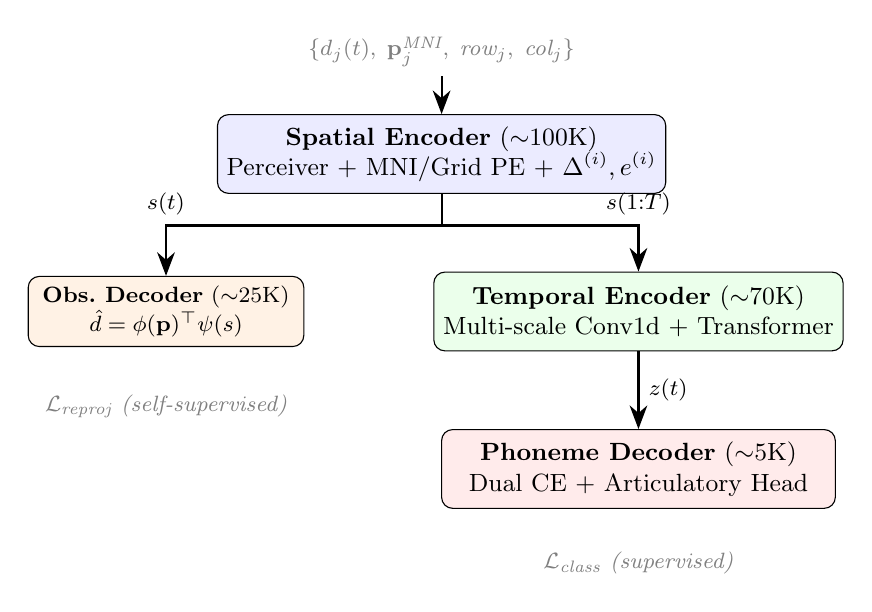
\begin{tikzpicture}[
  box/.style={draw, rounded corners, minimum width=5cm, minimum height=1cm, align=center, font=\small},
  smallbox/.style={draw, rounded corners, minimum width=3.5cm, minimum height=0.8cm, align=center, font=\footnotesize},
  arrow/.style={-{Stealth[length=3mm]}, thick},
  label/.style={font=\footnotesize\itshape, text=gray}
]

\node[box, fill=blue!8] (spatial) at (0, 0) {\textbf{Spatial Encoder} (${\sim}$100K)\\Perceiver + MNI/Grid PE + $\Delta^{(i)}, e^{(i)}$};

\node[smallbox, fill=orange!10] (obs) at (-3.5, -2) {\textbf{Obs.\ Decoder} (${\sim}$25K)\\$\hat{d} = \phi(\bfp)^\top\psi(s)$};

\node[box, fill=green!8] (temporal) at (2.5, -2) {\textbf{Temporal Encoder} (${\sim}$70K)\\Multi-scale Conv1d + Transformer};

\node[box, fill=red!8] (phoneme) at (2.5, -4) {\textbf{Phoneme Decoder} (${\sim}$5K)\\Dual CE + Articulatory Head};

\node[label] (input) at (0, 1.3) {$\{d_j(t),\; \bfp_j^{\text{MNI}},\; \text{row}_j,\; \text{col}_j\}$};

\draw[arrow] (input) -- (spatial);
\draw[arrow] (spatial.south) -- ++(0,-0.4) -| (obs.north) node[midway, above, font=\footnotesize] {$s(t)$};
\draw[arrow] (spatial.south) -- ++(0,-0.4) -| (temporal.north) node[midway, above, font=\footnotesize] {$s(1{:}T)$};
\draw[arrow] (temporal) -- (phoneme) node[midway, right, font=\footnotesize] {$z(t)$};

\node[label] at (-3.5, -3.2) {$\mathcal{L}_{\text{reproj}}$ (self-supervised)};
\node[label] at (2.5, -5.2) {$\mathcal{L}_{\text{class}}$ (supervised)};

\end{tikzpicture}
\end{center}

\begin{equation}
\boxed{\mathcal{L} = \mathcal{L}_{\text{class}} + \lambda \cdot \mathcal{L}_{\text{reproj}}}
\end{equation}

\begin{table}[ht]\centering\small
\begin{tabular}{@{}lrl@{}}
\toprule
\textbf{Module} & \textbf{Params} & \textbf{Role}\\
\midrule
Spatial encoder & ${\sim}$100K & Invert observation function\\
Observation decoder & ${\sim}$25K & Forward model (reprojection)\\
Temporal encoder & ${\sim}$70K & Dynamics modeling\\
Phoneme decoder & ${\sim}$5K & Classification\\
\midrule
\textbf{Total shared} & ${\sim}$\textbf{200K} &\\
Per-patient ($\times 10$) & 670 & Registration + identity\\
\textbf{Grand total} & ${\sim}$\textbf{201K} & (cf.\ current pipeline: 122K)\\
\bottomrule
\end{tabular}
\end{table}


%% ====================================================================
%%  PART IV: TRAINING AND EVALUATION
%% ====================================================================

\part{Training, Evaluation, and Next Steps}

\section{Training Pipeline}

\subsection{Phase 1: Source patient training (supervised + reprojection)}

9 source patients, ${\sim}1315$ labeled trials. Each batch:
\begin{enumerate}[leftmargin=2em]
\item Spatial encoding: construct tokens, mask 20--40\% electrodes, Perceiver $\to s(t)$.
\item Reprojection: decoder predicts all electrodes (including masked); $\mathcal{L}_{\text{reproj}}$.
\item Temporal encoding: $s(1{:}T) \to$ multi-scale $\to$ transformer $\to z(t)$.
\item Classification: dual head $\to \mathcal{L}_{\text{class}}$.
\item Total: $\mathcal{L} = \mathcal{L}_{\text{class}} + \lambda \mathcal{L}_{\text{reproj}}$ ($\lambda$: 0.5 $\to$ 0.1 annealed).
\end{enumerate}

AdamW, differential LR (shared 1e-3; virtual positions/patient $\Delta$ 3e-4), cosine schedule, warmup 20 epochs, early stopping patience 7.

\textbf{Optional}: alternate labeled batches (both losses) with unlabeled batches from continuous recordings or Lexical patients (reprojection only).

\subsection{Phase 2: Target adaptation (LP-FT)}

Per CV fold on S14 (153 trials, 5-fold grouped-by-token):
\begin{enumerate}[leftmargin=2em]
\item \textbf{Linear probe}: freeze encoder, train decoder + $\Delta^{(\text{S14})} + e^{(\text{S14})}$.
\item \textbf{Fine-tune}: unfreeze encoder at 0.1$\times$ LR.
\end{enumerate}

\subsection{Phase 3 (optional): Reprojection pre-training}

Pre-train spatial encoder + observation decoder on all available data (continuous recordings + Lexical patients) using $\mathcal{L}_{\text{reproj}}$ only. No labels needed. Then initialize Phase~1 from pre-trained weights.


\section{Evaluation}

PER via edit distance, grouped-by-token 5-fold CV. Full recipe: weighted $k$-NN ($k{=}10$, cosine), TTA 16, dual head, best-of per fold, source $k$-NN at $0.5\times$ weight.

\subsection{Key ablations}

\begin{table}[ht]\centering\small
\begin{tabular}{@{}clp{7cm}@{}}
\toprule
\textbf{ID} & \textbf{Ablation} & \textbf{Question}\\
\midrule
A1 & MNI PE present/absent & Do MNI coordinates help? (central question)\\
A2 & All patients vs.\ S14 only & Is the 0.76 wall S14-specific?\\
A3 & $\Delta$ / $e$ / both / neither & Which per-patient params matter?\\
A4 & $L \in \{4, 8, 16, 32\}$ & How many virtual electrodes?\\
A5 & $\lambda \in \{0, 0.01, 0.1, 0.5\}$ & Does reprojection loss help?\\
A6 & $+$ Duraivel cross-task data & Does more data help? (independent of architecture)\\
\bottomrule
\end{tabular}
\end{table}


\section{Data Paths}

\textbf{Highest priority (lowest risk):} Cross-task pooling from Duraivel 2025---same tokens, same phonemes, overlapping patients, compatible preprocessing.

\textbf{Medium priority:} MNI coordinate sourcing (BioImage Suite / Brainlab / ECoG\_Recon on Box). Hard dependency for the Perceiver architecture.

\textbf{Lower priority:} Continuous recording extraction + VAD curation for Phase~3 SSL.


\section{Success Criteria}

\begin{table}[ht]\centering\small
\begin{tabular}{@{}lp{9cm}@{}}
\toprule
\textbf{Level} & \textbf{Criterion}\\
\midrule
Minimum & A1: Perceiver + MNI outperforms Perceiver without MNI by ${\geq}2\pp$ on S14\\
Target & PER $<$ 0.740 on S14 (exceeds per-patient supervised 0.737)\\
Strong & Population-level improvement across all patients\\
Interpretability & Virtual electrodes cluster over vSMC; $\Delta^{(i)}$ larger for tumor patients; $\phi(\bfp)$ recovers somatotopy\\
\bottomrule
\end{tabular}
\end{table}


\section{Summary}

This document formalizes cross-patient speech decoding as \textbf{multi-view neural field reconstruction}: multiple patients observe the same cortical dynamics from different electrode positions, analogous to multiple cameras observing the same 3D scene. The shared observation function $g(\bfp, \bfz)$ is the somatotopic map; patient-specific parameters ($\Delta$, $e$) are camera calibration; the reprojection loss trains spatial alignment without labels.

The Neural Field Perceiver implements this framework: Perceiver cross-attention with MNI distance bias inverts the observation function, a bilinear decoder implements it forward for reprojection, multi-scale temporal transformer models articulatory dynamics, and per-position classification decodes the phoneme sequence. The architecture uses ${\sim}200$K shared parameters and 67 per patient, directly mapping every component to the observation equation.

\end{document}
